\chapter{Optimized Scheduling}
\label{chap:mode_mapping}

%%%%%%%%%%%%%%%%%%%%%%%%%%%%%%%%%%%%%
%%%%%%%%%%%%%%%%%%%%%%%%%%%%%%%%%%%%%
%%%%%%%%%%%%   SECTION   %%%%%%%%%%%%
%%%%%%%%%%%%%%%%%%%%%%%%%%%%%%%%%%%%%
%%%%%%%%%%%%%%%%%%%%%%%%%%%%%%%%%%%%%
\section{Scheme 3}
\label{sec:mm:scheme4}
According to the A/A Mode processing chain, only Correlation Processing is dependent on the results of the 8 bursts of a dwell. The burst processing chain except the correlation processing has no dependency and can therefore performed independently. The previous 7 bursts. Rest of the processing steps do not have any dependency, thus can be performed independently. The final Correlation Processing shall be computed serially. Space Partition configuration is adopted for Scheme-3 implementation.

\subsection{Hypothesis}
\textbf{\textsl{A Burst shall be processed as soon as a core receives it. This avoids unnecessary waiting time to receive a complete Dwell (8 Bursts) data.}}\\[0.2cm]
In case of the baseline analysis, as illustrated in Figure \ref{fig:mm:scheme4_data_distribution}, beam-forming of the first burst will start only after receiving a complete dwell. Though the first burst is ready for Beam-forming, redundant time is spent in waiting for the complete dwell data. This applies to the Pulse Compression, FFT, and CFAR processing also.

Scheme-3 exploits the fact that every burst can be processed independently until the Thresholding and Detection stage. Every burst is sent to an individual core to process them conveniently as soon as they are received. This saves waiting time during Data receive period, Beam-forming, Pulse compression, FFT and CFAR processing. Nothing has changed in terms of Correlation Processing, hence it will not contribute to the latency reduction.

\subsection{Scheduling Scheme}
As shown in Figure \ref{fig:mm:scheme4_aa_mode_mapping}, CPU1...6 are allocated for burst processing and CPU7 executes four instances of Correlation Processing in four cores, performing one instance per core. Burst processing comprises of Beam-forming, Pulse Compression, FFT and CFAR processing. A burst processing CPU gets four bursts and executes one instance of burst processing per core.

\begin{tabular}{rl}
	No.of cores for burst processing: & 6 x 4 = 24 \\
	No.of cores for correlation processing: & 1 x 4 = 4 \\
	Data distribution-burst processing: & One burst per core \\
	Data distribution-correlation processing: & One dwell per core \\
\end{tabular}
%\FloatBarrier 

\begin{figure}[h!]
	\centering
	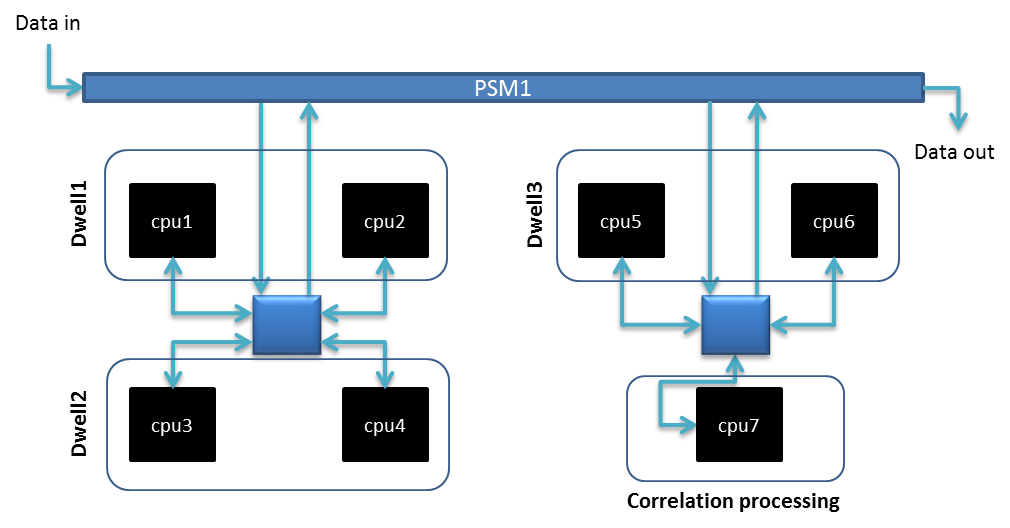
\includegraphics[width=140mm]{figures/scheme4_aa_mode_mapping}
	\caption{Scheduling Scheme}
	\label{fig:mm:scheme4_aa_mode_mapping}
\end{figure}

\vspace*{0.2cm}
\noindent
The received A/A mode raw data will be processed as follows

\begin{enumerate}
\item PSM1 routes each burst data to each core starting from core1 of CPU1 to core4 of CPU6 in round robin fashion.
\item Each core in the CPU1...6 performs burst processing followed by storing the results in SDRAM.
\item In a burst processing CPU, a core completing the processing steps last will transfer all the cores(Core\#1...\#4) results to the CPU7 for correlation processing. This avoids frequent communication between burst processing CPUs and correlation processing CPU. The data passed to the CPU7 is alarm list and their related information, which is smaller in size and assumed that it requires only 0.01ms to transfer.
\item Each core of the CPU7 waits for processed 8 burst data, and then performs Correlation Processing followed by sending out the target detections to PSM1.
\item PSM1 directs the results to tracking processor or display processor. Scheduling scheme is shown in Figure \ref{fig:mm:scheme4_data_distribution}.
\end{enumerate}

\begin{figure}[h!]
	\centering
	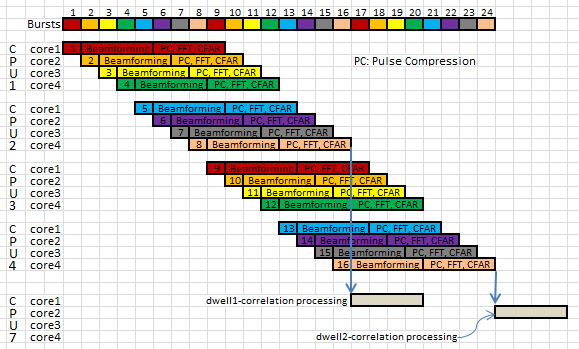
\includegraphics[width=140mm]{figures/scheme4_data_distribution.png}
	\caption{Scheduling Scheme}
	\label{fig:mm:scheme4_data_distribution}
\end{figure}

\begin{figure}[h!]
	\centering
	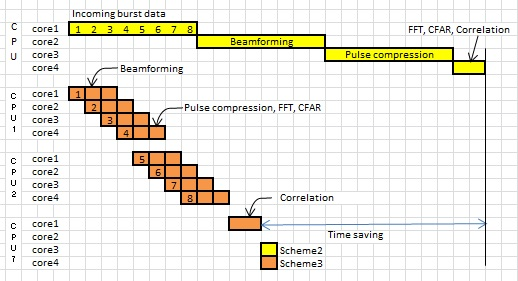
\includegraphics[]{figures/scheme4_comparison}
	\caption{Comparison of Scheduling Schemes}
	\label{fig:mm:scheme4_comparison}
\end{figure}

Another difference between Scheme-1 and Scheme-3 is the amount of data processed by a CPU. Scheme-1 performs 8 bursts processing whereas Scheme-3 performs 4 bursts processing per CPU. This decreases memory requirement and memory transfer bandwidth compared to the Scheme-1.

\subsection{Processing Latency}
\label{ss:mm:scheme4:latency}
Processing latency is measured on a real hardware clocked 1GHz and the results are scaled down to 800MHz. Data transfer time of 0.02ms is assumed between CPU1...6 and CPU7. Processing latency calculations of every core is shown in Appendix \ref{app:sch3:calc}. Figure \ref{fig:mm:scheme3_req_time} shows the latency components corresponds to PRF1, Look Direction-1 of one Burst.  Table \ref{fig:mm:scheme4_elapsed_time} summarizes the time required to process one burst until Thresholding and Detection stage.

\begin{figure}[h!]
	\centering
	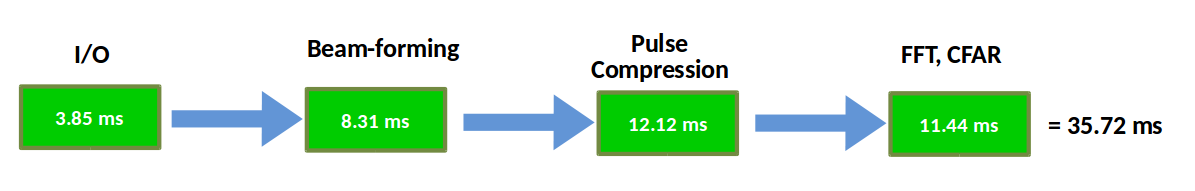
\includegraphics[width=145mm]{figures/scheme3_req_time}
	\caption{Burst Processing time for PRF1, Look Direction-1}
	\label{fig:mm:scheme3_req_time}
\end{figure}

The stated values in the table say that the look direction-1, PRF1 needs 35.72ms time to complete the execution from the moment a core starts receiving a burst. Elapsed wall clock time to process burst by burst is listed as \textsl{Time spent[ms]}. Example calculations for the look direction-1 are explained here with reference to the Figure \ref{fig:mm:scheme4_timeline_burst_proc}. A core waits for the pre-defined burst data to be received, i.e. a core processing PRF8 should wait till the PRF1...7 are distributed by the iCON. Burst receive time are derived from the Radar characteristics (see Chapter \ref{ss:aa_mode:radar_char}).

\begin{table}[h!]
	\centering
	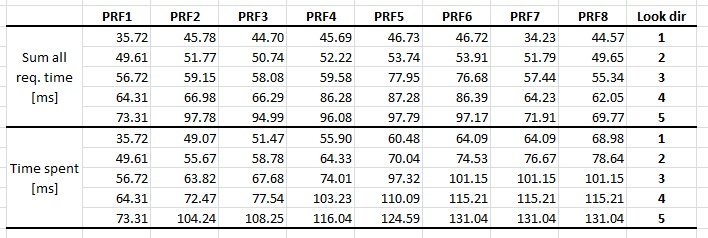
\includegraphics[width=140mm]{figures/scheme4_elapsed_time}
	\caption{Processing Time}
	\label{fig:mm:scheme4_elapsed_time}
\end{table}

\begin{figure}[h!]
	\centering
	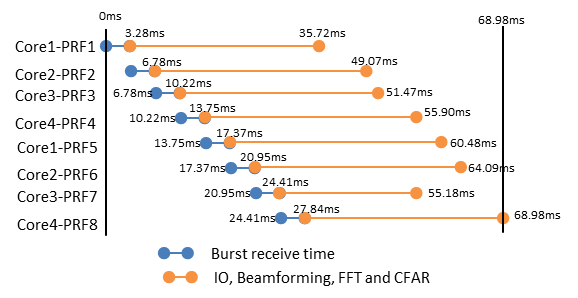
\includegraphics[width=130mm]{figures/scheme4_timeline_burst_proc}
	\caption{Elapsed Time Calculation}
	\label{fig:mm:scheme4_timeline_burst_proc}
\end{figure}

%\setlength{\belowdisplayskip}{2pt} \setlength{\belowdisplayshortskip}{2pt}
%\setlength{\abovedisplayskip}{0pt} \setlength{\abovedisplayshortskip}{0pt}
\begin{align*}
	T_{el} &= MAX((T_{pb} + T_{ex}), T_{el})\\
	PRF1 &= MAX((0 + 35.72), 0) = 35.72 \: ms\\
	PRF2 &= MAX((3.28 + 45.78), 35.72) = 49.07 \: ms \\	 
	PRF3 &= MAX((3.28 + 3.50 + 44.7),49.07) = 51.47 \: ms \\
		& \: \: . \\
		& \: \: . \\
		& \: \: . \\	
	PRF8 &= MAX((3.28 + 3.50 + 3.44 + 3.53 + 3.63 + 3.57 + 3.46 + 44.57), 64.09) \\
		&= 68.98 \: ms	\stepcounter{equation}\tag{\theequation}
\end{align*}
\noindent 
\textbf{Legend}\\
\tab $T_{el}:$ Elapsed time \\
\tab $T_{ex}:$ Execution time \\
\tab $T_{pb}:$ Previous burst receive time\\


Data transfer time of 0.02ms between burst processing CPUs and correlation processing CPU, and 0.2ms between correlation processing CPU and tracking/display processor is assumed.
\begin{align*}
	T_{l} &= T_{bp} + T_{dt} + T_{cp} + T_{tr}  \\
		&= 68.98 + 0.02 + 43.34 + 0.2 = 112.5 \: ms  \stepcounter{equation}\tag{\theequation}
\end{align*}
\noindent 
\textbf{Legend}\\
\tab $T_{l}:$ Processing latency \\
\tab $T_{bp}:$ Burst processing time \\
\tab $T_{dt}:$ Data transfer time from CPU1...6 to CPU7\\
\tab $T_{cp}:$ Correlation processing time \\
\tab $T_{tr}:$ Result transfer time from CPU7 to Tracking/Display processor \\

The processing latency between 112.52ms and 174.58ms are achieved depending on the look direction. Table \ref{tbl:mm:scheme4_latency} lists the processing latency of every look direction.
\begin{table}[h!]
	\centering
	\begin{tabular}{|c|l|l|l|} 
	 \hline
	 \textbf{Look direction} & \textbf{Dwell time[ms]} & \textbf{Latency[ms]} & \textbf{\#Dwells transmitted} \\
	 \hline
	 1 & 27.84 & 112.52 & 4.04 \\ \hline
	 2 & 33.07 & 122.18 & 3.69 \\ \hline
	 3 & 39.17 & 144.69 & 3.69 \\ \hline
	 4 & 46.20 & 158.75 & 3.44 \\ \hline
	 5 & 54.26 & 174.58 & 3.22 \\ \hline
	\end{tabular}
	\caption{Processing Latency}
	\label{tbl:mm:scheme4_latency}
\end{table}
\FloatBarrier

\subsection{CPU Utilization}
\label{ss:mm:scheme4:cpu_load}
\subsubsection{Burst Processing CPUs}
CPU utilization is the ratio of processing time to the available time. 6 CPUs are involved in A/A mode processing; meaning 24 cores are processing 24 burst (3 Dwell) data. Available time is 3x Dwell time. Utilization of each core per look direction is listed in Appendix \ref{fig:mm:scheme4_util}. Summarized utilization result is presented in Figure \ref{sch3:chrt:cpu_util}. From the figure, it can be seen that the maximum core utilization reaches up to 66\%.
\begin{figure}[h!]
\centering
\resizebox {10cm} {!} {
		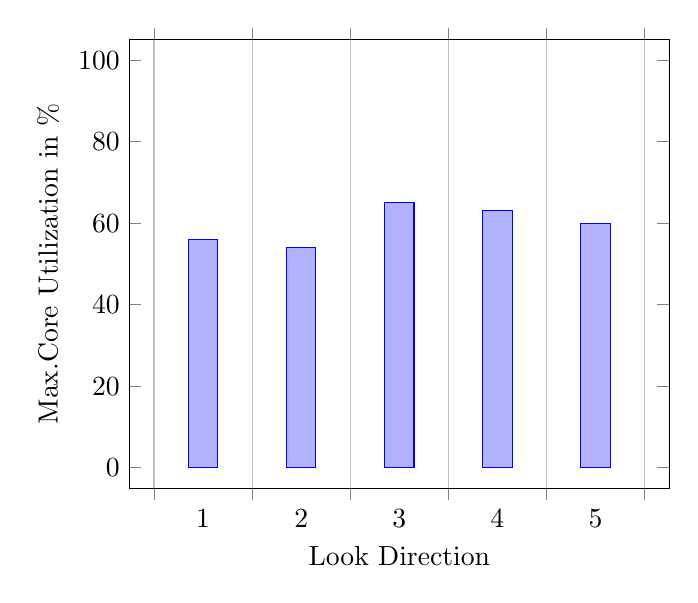
\begin{tikzpicture}{}
		\begin{axis}[
			x tick label style={/pgf/number format/1000 sep=},
			ylabel=Max.Core Utilization in \%,
			xlabel=Look Direction,
			enlargelimits=0.05,
			legend style={at={(0.5,-0.1)},
			anchor=north,legend columns=-1},
			ybar interval=0.3,
			ymin=0,ymax=100,
			]
		\addplot
			coordinates {(1, 56) (2, 54) (3, 65) (4, 63) (5, 60) (6, 19.16)};
		\end{axis}
		\end{tikzpicture}
}
\caption{CPU Utilization - Burst Processing CPUs}
\label{sch3:chrt:cpu_util}
\end{figure}	
	
\subsubsection{Correlation Processing CPU}
\label{mm:SSS:scheme4:corr_cpu_util}
Correlation processing time values are listed in Appendix \ref{app:sch4:corr_cpu_util}. Processing time of one Dwell on a single core is given in Figure \ref{fig:mm:scheme4_corr_components}.

\begin{figure}[h!]
	\centering
	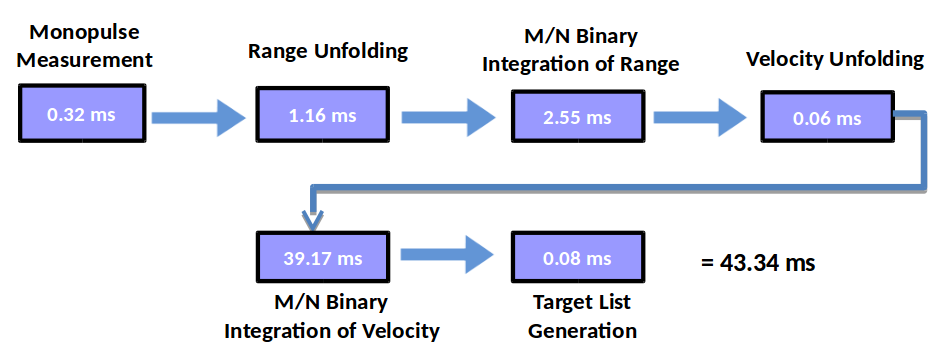
\includegraphics[width=120mm]{figures/scheme4_corr_components}
	\caption{Correlation Processing Time on a Single Core}
	\label{fig:mm:scheme4_corr_components}
\end{figure}

Every core of the correlation processing CPU is in idle state until it receives the results of 8 burst data from CPU1...6. Then it continues processing for 43.34ms before returning to idle state. Dwells are distributed to 4 cores of the CPU7 in round robin manner. Core\#1 of the CPU7 can start processing as soon as 8 bursts of a Dwell are received. 1ms delay is assumed between burst processing CPUs sending out the data and CPU7 starts processing. From the Table \ref{fig:mm:scheme4_elapsed_time}, look direction-1 needs 68.98ms to do burst processing. Until this time, Core\#1 of the CPU7 is in idle state. Correlation processing takes place for the next 43.34ms in Core\#1 followed by waiting for the next set Dwell5 data. Dwell5 will be supplied to the burst processing CPUs at 115.3ms (4 x 27.84ms) by the incoming data stream. Received Dwell5 data will be fed to CPU7 after 68.98ms (processing) + 1ms (transfer). From Figure \ref{sch3:chrt:corr_cpu_util}, peak utilization of the CPU7 is 39\%, belongs to the look direction-1. Utilization calculation for the look direction-1 is depicted in Figure \ref{fig:mm:scheme4_corr_cpu_util_pic}, and the utilization of Core\#1 is derived as follows.

\begin{align*}
	U_{1} &= \frac{T_{cp}}{ T_{cp} + T_{i}} = \frac{43.34}{43.34 + 69.98} = 38\% \\[0.4cm]
	T_{ndi} &= I_{d5} + T_{bp} \\
	&= 4 * 27.84 + 69.98 =181.3 \: ms\\
	T_{i} &= T_{ndi} - T_{ldo} \\
	&= 181.33 - (69.98 + 43.34) = 68.01 \: ms \\
	U_{5} &= \frac{43.34}{43.34 + 68.01} = 39\%  \stepcounter{equation}\tag{\theequation}
\end{align*}
\noindent 
\textbf{Legend}\\
\tab $U_{1}:$ Utilization at Dwell1 \\
\tab $T_{cp}:$ Correlation processing time \\
\tab $T_{i}:$ Idle time \\
\tab $T_{ndi}:$ Next Dwell in \\
\tab $T_{ldo}:$ Last Dwell out \\
\tab $T_{bp}:$ Burst processing time \\
\tab $I_{d5}:$ Dwell5 input at burst processing CPU 

\begin{figure}[h!]
	\centering
	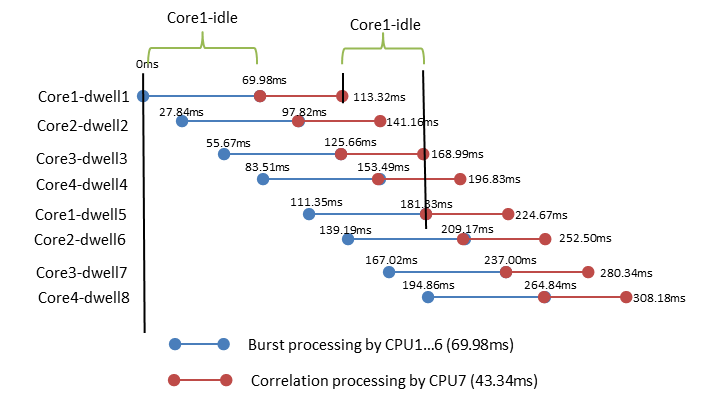
\includegraphics[width=160mm]{figures/scheme4_corr_timeline}
	\caption{Core\#1 - Idle Time, While Processing Look Direction-1 }
	\label{fig:mm:scheme4_corr_cpu_util_pic}
\end{figure}

\begin{figure}[h!]
\centering
\resizebox {10cm} {!} {
		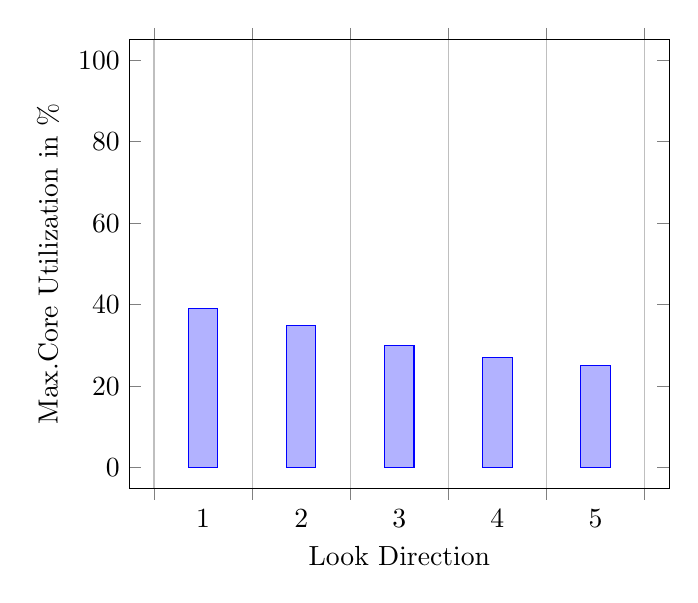
\begin{tikzpicture}{}
		\begin{axis}[
			x tick label style={/pgf/number format/1000 sep=},
			ylabel=Max.Core Utilization in \%,
			xlabel=Look Direction,
			enlargelimits=0.05,
			legend style={at={(0.5,-0.1)},
			anchor=north,legend columns=-1},
			ybar interval=0.3,
			ymin=0,ymax=100,
			]
		\addplot
			coordinates {(1, 39) (2, 35) (3, 30) (4, 27) (5, 25) (6, 19.16)};
		\end{axis}
		\end{tikzpicture}
}
\caption{CPU Utilization - Burst Processing CPUs}
\label{sch3:chrt:corr_cpu_util}
\end{figure}

Utilization drops for ascending look direction, since look direction 5 has longest data receive time and processing time but maximum target detections are same for all the look directions. 
\FloatBarrier

\subsection{Memory Transfer Bandwidth}
\label{ss:mm:scheme4:bw_util}
Lowest recorded memory transfer bandwidth by running the STREAM benchmark as a background task is listed in Table \ref{tbl:mm:scheme4_mem_bw} 
Peak memory transfer bandwidth of the Radar application is measured as 39.4\% of the available 1048MiB/s.

\begin{table}[h!]
	\centering
	\begin{tabular}{|l|l|} 
	 \hline
	 \textbf{Function} & \textbf{Best Rate [MiB/s]} \\
	 \hline
	 Copy & 635.0 \\ \hline
	\end{tabular}
	\caption{Lowest Recorded Memory Transfer Bandwidth of the STREAM Benchmark}
	\label{tbl:mm:scheme4_mem_bw}
\end{table}

\begin{align*}
\label{aa:scheme4:mem_bw}
	BW_{p} &= BW_{i} - BW_{l} \\
	&= 1048 - 635 = 413 \: MiB/s \\
	&= \frac{413}{1048} = 39.4 \% \stepcounter{equation}\tag{\theequation} 
\end{align*}
\noindent 
\textbf{Legend}\\
\tab $BW_{p}:$ Peak bandwidth of the optimized scheme \\
\tab $BW_{i}:$ Idle bandwidth of the Nitrogen6X board \\
\tab $BW_{l}:$ Lowest recorded bandwidth \\

\subsection{Memory Utilization}
\label{ss:mm:scheme4:mem_util}
Peak memory utilization of the optimized scheme (Scheme-3) is measured as 0.9\% of the available 879MiB memory. Memory utilization is sampled 10 times a second until the A/A Mode sequence is running. Figure \ref{fig:mm:scheme4_mem_util} shows memory utilization footprint in a graphical view.

\begin{figure}[h!]
	\centering
	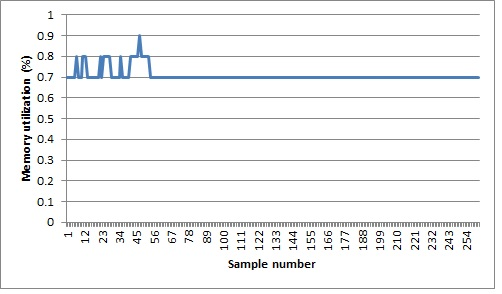
\includegraphics[width=100mm]{figures/scheme4_mem_util}
	\caption{Scheme-3, Memory Utilization Footprint}
	\label{fig:mm:scheme4_mem_util}
\end{figure}
\FloatBarrier

\subsection{Summary}
\label{ss:mm:scheme4:summary}
Scheme-3 has 4x Dwell time latency, 66\% CPU utilization, 39.4\% memory transfer bandwidth utilization and 1\% memory utilization. CPU utilization can be improved by adding more DGPMs. An IMA processor architecture can have upto 6 DGPMs comprising of 24 CPUs. Scheme-3 has utilized 28 cores of 7 CPUs, while rest of the 17 CPUs can be used for other purpose including A/G mode processing. A comparison of Scheme-1, Acceptable values and Scheme-3 is given below.

\begin{table}[h!]
	\centering
	\begin{tabular}{|l|l|l|l|} 
	 \hline
	 \textbf{Parameter} & \textbf{Scheme-1} & \textbf{Acceptable Values} & \textbf{Scheme-3}\\
	 \hline
	 Dwells transmitted &  14.96 & 2 & 4.04 \\ \hline
	 CPU utilization & 75.5\% & \textless 50\% & 66\% \\ \hline
	 Memory utilization & 7\% & \textless 50\%  & 1\% \\ \hline
	 Memory transfer bandwidth & NA & \textless 50\% & 41\%  \\ \hline
	\end{tabular}
	\caption{Comparison of Scheme-1 vs Acceptable Values vs Scheme-3}
	\label{tbl:mm:scheme4_comparison}
\end{table}

\clearpage
%%%%%%%%%%%%%%%%%%%%%%%%%%%%%%%%%%%%%
%%%%%%%%%%%%%%%%%%%%%%%%%%%%%%%%%%%%%
%%%%%%%%%%%%   SECTION   %%%%%%%%%%%%
%%%%%%%%%%%%%%%%%%%%%%%%%%%%%%%%%%%%%
%%%%%%%%%%%%%%%%%%%%%%%%%%%%%%%%%%%%%
\section{Scheme 4}
\label{sec:mm:scheme5}
Space Partition configuration is adopted for Scheme-4 implementation.
\subsection{Hypothesis}
\textsl{\textbf{Burst processing of each channel($S_{S},S_{G},S_{AZ},S_{EL}$) shall be performed in parallel as long as they are independent. This eliminates waiting time while processing other channel data. }}
\begin{compactitem}
\item Taking a closer look into the processing chain in Chapter \ref{sec:bg_related_work:proc_chain}, revels that a burst data has 4 channel processing namely Sum, Guard, Azimuth and Elevation.  These 4 channels do not have data dependency, allowing for parallel execution. In Scheme-3, Core\#1 does Beam-forming of one Burst serially, which comprises of computing Beam-forming for Sum channel, Azimuth channel and Elevation channel one after another. Scheme-4 proposes to perform them in parallel, leading to faster execution.
Data dependency diagram for A/A mode processing is shown in Figure \ref{fig:mm:scheme5_data_path}.

\begin{figure}[h!]
	\centering
	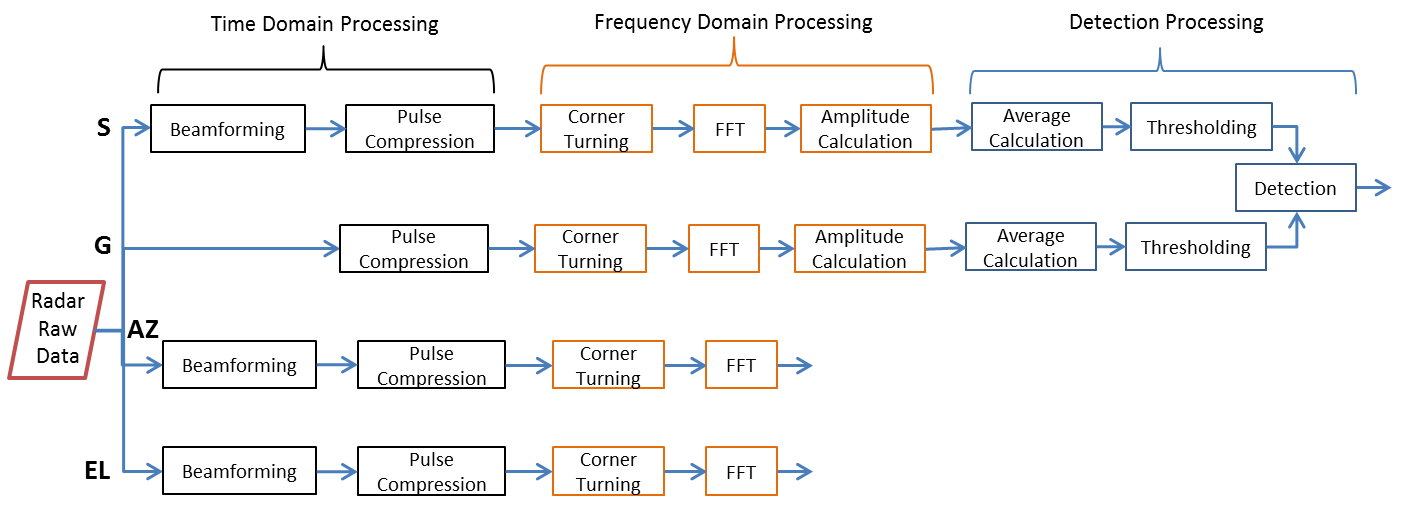
\includegraphics[width=160mm]{figures/scheme5_data_path}
	\caption{A/A Mode - Data Dependency of the Radar Application}
	\label{fig:mm:scheme5_data_path}
\end{figure}
Note: The data dependency diagram does not consider constant table values such as Sum channel beam-forming vector, Azimuth channel beam-forming vector, etc, as they are pre-calculated and available at any point of time.

\item Correlation processing shall be optimized to bring down the execution time.
\end{compactitem}

\subsection{Scheduling Scheme}
\label{ss:mm:scheme5:data_distribution}
Four channel processing are done by 4 cores of a CPU. CPU1...12 gets one burst each. CPU13 and CPU14 are allocated for correlation processing. 
PSM1 routs the Radar raw data to the respective DGPMs. Burst results are sent to PSM1 by the CPUs 1..12. PSM1 stores the burst result until 8 burst results are received. Then 8 burst results are sent to the cores of CPU13 and CPU14 in round robin manner. The DGPMs and PSM are arranged as shown in Figure \ref{fig:mm:scheme5_mode_mapping} and the data distribution is illustrated in Figure \ref{fig:mm:scheme5_data_distri}.

\begin{figure}[h!]
	\centering
	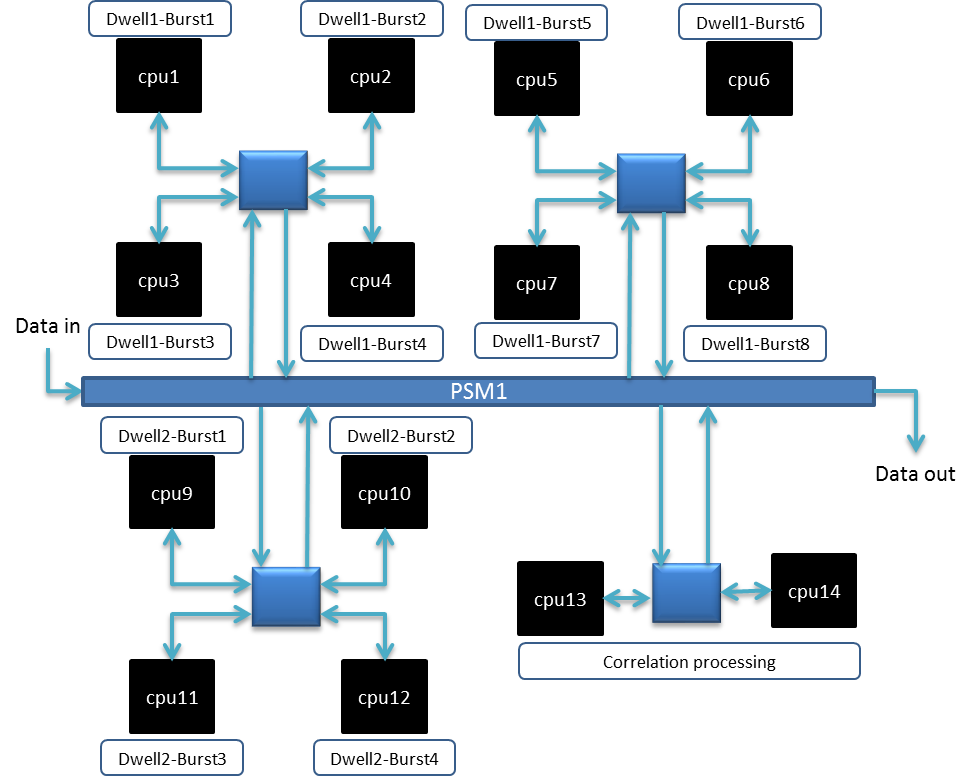
\includegraphics[width=130mm]{figures/scheme5_mode_mapping}
	\caption{Scheduling Scheme}
	\label{fig:mm:scheme5_mode_mapping}
\end{figure}

\begin{figure}[h!]
	\centering
	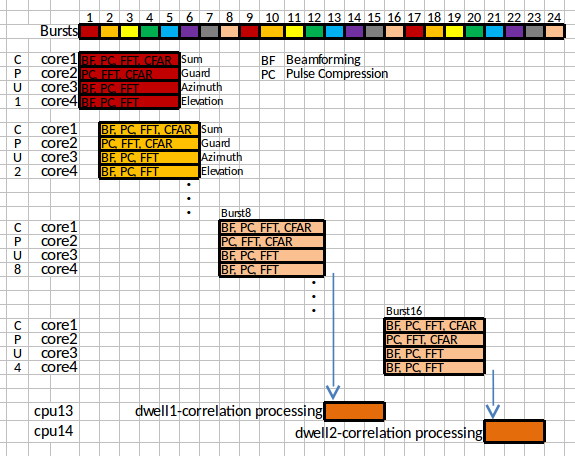
\includegraphics[width=130mm]{figures/scheme5_data_distri}
	\caption{Scheduling Scheme}
	\label{fig:mm:scheme5_data_distri}
\end{figure}

\begin{figure}[h!]
	\centering
	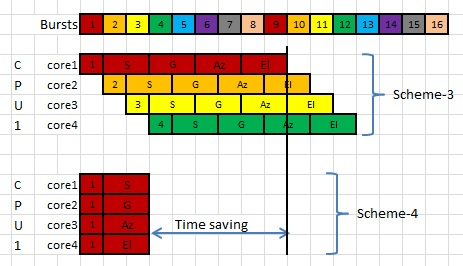
\includegraphics[width=95mm]{figures/scheme5_time_saving}
	\caption{Scheme-3 vs Scheme-4}
	\label{fig:mm:scheme5_time_saving}
\end{figure}

In terms of burst processing, every CPU in Scheme-3 performs computation on 4 burst data, whereas a CPU in Scheme-4 does computations on one burst. Single burst is placed in the shared memory, so that all the four cores can access them. CPU1 gets the first burst. Core1 of the CPU1 performs Beamforming, Pulse Compression, FFT and CFAR processing of Sum channel on the burst data. Rest of the three cores repeat the same for Guard channel, Azimuth and Elevation channel processing simultaneously. It results in approximately 4x reduced memory requirement than Scheme-3. A comparison of Scheme-3 and Scheme-4 is shown in Figure \ref{fig:mm:scheme5_time_saving}.
\FloatBarrier

Correlation processing requires 43.34ms (see Chapter \ref{mm:SSS:scheme4:corr_cpu_util}) to process one Dwell data. Dwell time of the look direction-1 is 27.84ms. Correlation processing itself consumes 1.5x Dwell transmission time. Best result cannot be achieved without optimizing the correlation processing. Pictorial view of the Correlation processing execution time is shown in Figure \ref{fig:mm:corr_proc_pie}.

\begin{figure}[h!]
	\centering
	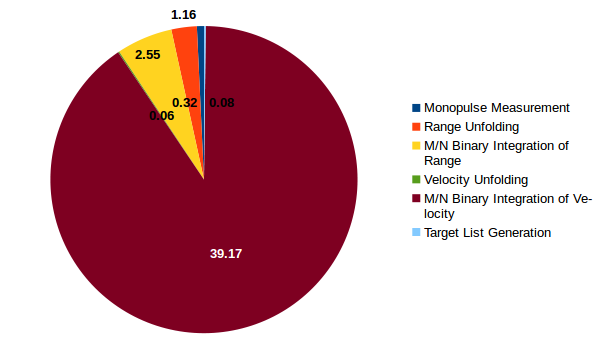
\includegraphics[width=120mm]{figures/corr_proc_pie}
	\caption{Correlation Processing - Processing Time in [ms]}
	\label{fig:mm:corr_proc_pie}
\end{figure}

According to the derivations of measurement time, M/N Binary Integration of Velocity(BIV) consumes 39.16ms of total 43.34ms. It is a good candidate for optimization. M/N BIV is implemented in \verb|C| according to the pseudo-code shown in Appendix \ref{app:sch4}, and the execution time is measured as 31.72ms when four instances are running on four cores. The loop iterations(Algorithm \ref{mm:biv:pseudo_code}, Line 3) of a single instance of M/N BIV are independent of the previous loop processing and next loop processing. They are broken into four sub-loops to run on four cores of a CPU in parallel. 4x speed-up is achieved for M/N Binary Integration of Velocity, reducing execution time from 31.72ms to 7.93ms. Any correlation processing CPU in Scheme-4 processes one dwell data, on contrary to the 4 dwell data in Scheme-3. Scheduling scheme and time saving are shown in Figure \ref{fig:mm:scheme5_corr_dd}, data dependency is shown in Figure \ref{fig:mm:scheme5_corr_data_path}.

\begin{figure}[h!]
	\centering
	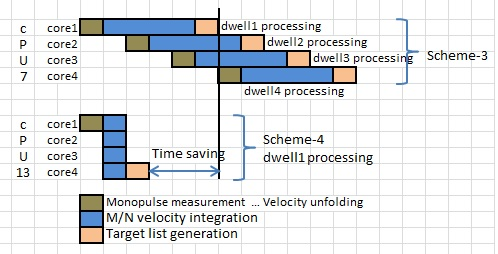
\includegraphics[width=95mm]{figures/scheme5_corr_dd}
	\caption{Comparison of Correlation Processing Schemes}
	\label{fig:mm:scheme5_corr_dd}
\end{figure}

\begin{figure}[h!]
	\centering
	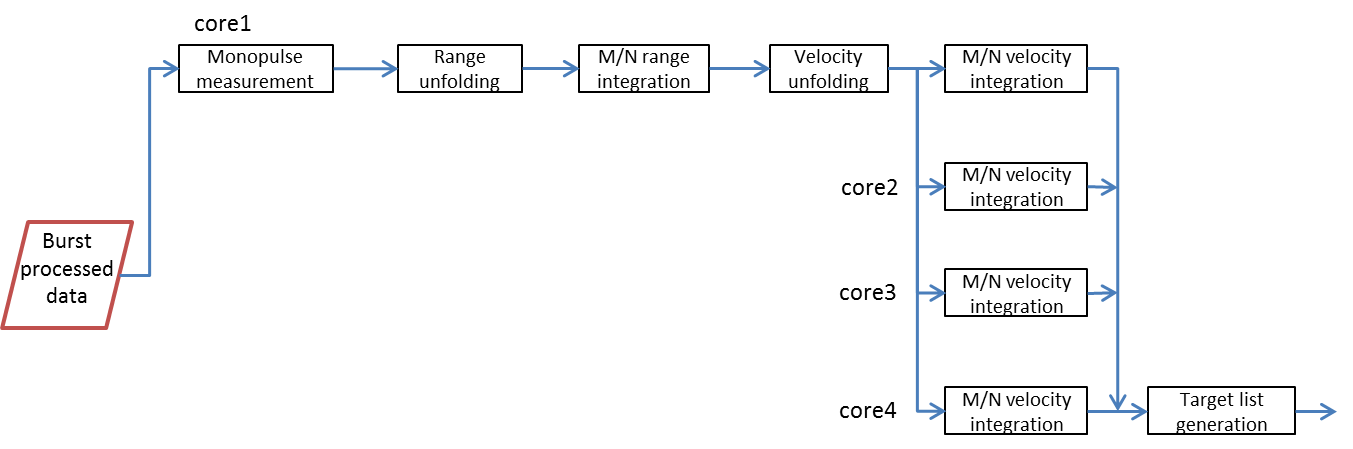
\includegraphics[width=140mm]{figures/scheme5_corr_data_path}
	\caption{Correlation Processing - Data Dependency and Scheduling Scheme}
	\label{fig:mm:scheme5_corr_data_path}
\end{figure}
At first, Core\#1 receives the dwell data for correlation processing, it does Monopulse measurement, Range unfolding, M/N range integration and Velocity unfolding serially. Afterwards, four threads are spawned to perform M/N BIV in parallel; each tread is allocated to a core. The thread completing M/N BIV last, will perform Target list generation followed by sending out the results to tracking/display processor via PSM1. Time delay of 0.02ms is assumed to spawn the threads and collect the results back. Resulting correlation processing time is calculated as follows. (Note: Execution time of the correlation processing steps can be seen in Figure \ref{fig:mm:scheme4_corr_calc})

\begin{align*}
\label{aa:scheme5:corr}
	T_{cp} &= T_{cp1} + T_{biv} + T_{tlg} +T_{ov} \\
	&= 4.09 + 7.93 + 0.02 + 0.02 = 12.06 \: ms \\ \stepcounter{equation}\tag{\theequation} 
\end{align*}
\noindent 
\textbf{Legend}\\
\tab $T_{cp1}:$ Monopulse measurement to Velocity unfolding processing time \\
\tab $T_{biv}:$ Time to process M/N BIV \\
\tab $T_{tlg}:$ Time to process Target list generation \\
\tab $T_{ov}:$ Overhead

\subsection{CPU Utilization}
\label{ss:mm:scheme5:cpu_load}
\subsubsection{Burst Processing CPUs}
Twelve CPUs are processing one burst each. Available time of a CPU is the time span between reception of two bursts to the CPU, which is 12x average burst time. Figure \ref{sch4:chrt:cpu_util} summarizes the CPU utilization for every look direction. Total time required to process one channel of a burst by a core is calculated as the sum of IO processing, Beam-forming, Pulse compression, FFT, CFAR, Thresholding, Detection and data copy time between SDRAM to the core. Detailed calculations can be found in appendix \ref{app:sch4_cpu_util}. As shown in the figure, it is implied that the peak CPU utilization reaches up to 50.8\%. Figure \ref{fig:mm:sch4_proc_time_chrt} shows the processing time of the Radar processing chain for Look direction-1, PRF1.

\begin{figure}[h!]
	\centering
	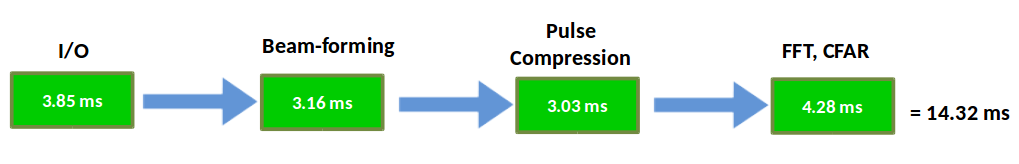
\includegraphics[width=140mm]{figures/sch4_proc_time_chrt}
	\caption{Burst Processing time for PRF1, Look Direction-1}
	\label{fig:mm:sch4_proc_time_chrt}
\end{figure}

\begin{figure}[h!]
\centering
\resizebox {10cm} {!} {
		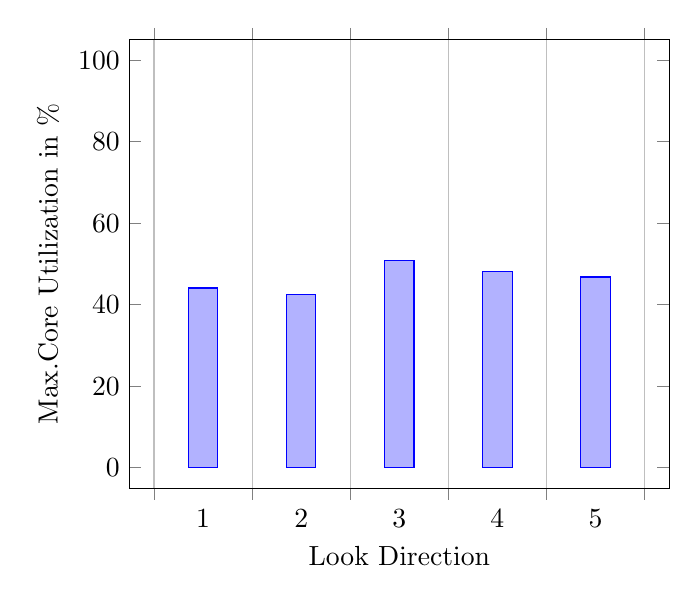
\begin{tikzpicture}{}
		\begin{axis}[
			x tick label style={/pgf/number format/1000 sep=},
			ylabel=Max.Core Utilization in \%,
			xlabel=Look Direction,
			enlargelimits=0.05,
			legend style={at={(0.5,-0.1)},
			anchor=north,legend columns=-1},
			ybar interval=0.3,
			ymin=0,ymax=100,
			]
		\addplot
			coordinates {(1, 44.1) (2, 42.6) (3, 50.8) (4, 48.1) (5, 46.8) (6, 19.16)};
		\end{axis}
		\end{tikzpicture}
}
\caption{CPU Utilization - Burst Processing CPUs}
\label{sch4:chrt:cpu_util}
\end{figure}

\subsubsection{Correlation Processing CPUs} 
The data processed by the CPU1...12 are grouped as Dwells and sent to CPU13 and CPU14 alternatively. Correlation processing CPUs are in idle state until they receive a dwell data then performs computation for 12.06ms followed by waiting for next set of burst results from the next Dwell. Time delay of 0.02ms is assumed to transfer results from burst processing CPUs to correlation processing CPUs. Timeline diagram is illustrated in Figure \ref{fig:mm:scheme5_corr_timeline}. Utilization calculations for the look direction-1 are listed below. 

\begin{figure}[h!]
	\centering
	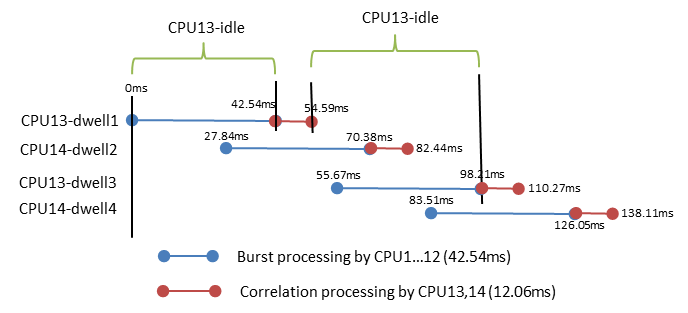
\includegraphics[]{figures/scheme5_corr_timeline}
	\caption{Look Direction-1, Utilization of the Correlation Processing CPU}
	\label{fig:mm:scheme5_corr_timeline}
\end{figure}

\begin{align*}
	U_{1} &= \frac{T_{cp}}{ T_{cp} + T_{i}} =  \frac{12.06}{12.06 + 42.54} = 22\% \\[0.4cm]
	T_{ndi} &= I_{d3} + T_{bp} \\
	&= 2 * 27.84 + 42.54 = 98.2 \: ms\\
	T_{i} &= T_{ndi} - T_{ldo} \\
	&= 98.2 - (12.06 + 42.54) = 43.6 \: ms \\
	U_{5} &= \frac{12.06}{12.06 + 43.6} = 22\%   \stepcounter{equation}\tag{\theequation}
\end{align*}

From the above calculation, it is seen that the peak utilization of the correlation processing CPU reaches upto 22\% when using two CPUs. Utilization of the Correlation processing CPUs for every look direction is given in Figure \ref{sch4:chrt:corr_cpu_util}.

\begin{figure}[h!]
\centering
\resizebox {10cm} {!} {
		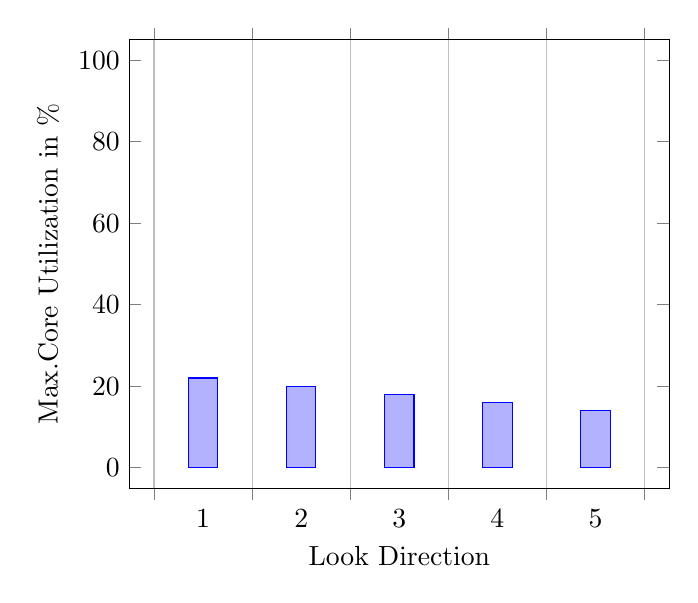
\begin{tikzpicture}{}
		\begin{axis}[
			x tick label style={/pgf/number format/1000 sep=},
			ylabel=Max.Core Utilization in \%,
			xlabel=Look Direction,
			enlargelimits=0.05,
			legend style={at={(0.5,-0.1)},
			anchor=north,legend columns=-1},
			ybar interval=0.3,
			ymin=0,ymax=100,
			]
		\addplot
			coordinates {(1, 22) (2, 20) (3, 18) (4, 16) (5, 14) (6, 19.16)};
		\end{axis}
		\end{tikzpicture}
}
\caption{CPU Utilization - Correlation Processing CPUs}
\label{sch4:chrt:corr_cpu_util}
\end{figure}

\subsection{Processing Latency}
\label{ss:mm:scheme5:latency}
Processing latency between 54.79ms and 88.17ms is achieved depending on the look direction, which is the time required for burst processing and correlation processing. Maximum Dwell time latency(\textsl{\#Dwells transmitted}) is 1.97x Dwell time contributed by the look direction-1. The processing latencies of the look direction-1...5 are listed below. 

\begin{table}[h!]
	\centering
	\begin{tabular}{|c|l|l|l|} 
	 \hline
	 \textbf{Look direction} & \textbf{Dwell time[ms]} & \textbf{Latency[ms]} & \textbf{\#Dwells transmitted} \\
	 \hline
	 1 & 27.84 & 54.79 & 1.97 \\ \hline
	 2 & 33.07 & 61.43 & 1.86 \\ \hline
	 3 & 39.17 & 69.10 & 1.76 \\ \hline
	 4 & 46.20 & 77.98 & 1.69 \\ \hline
	 5 & 54.26 & 88.17 & 1.62 \\ \hline
	\end{tabular}
	\caption{Processing Latency}
	\label{tbl:mm:scheme5_latency}
\end{table}

\subsection{Memory Utilization}
\label{ss:mm:scheme5:mem_util}
Memory utilization of Scheme-4 is measured as 0.5\% of the available 879MiB memory. Memory requirement is reduced since, one CPU is working on one burst data, whereas in Scheme-3, one CPU gets 4 burst data. Memory utilization footprint of the Scheme-4 implementation is shown in Figure \ref{fig:mm:scheme4_mem_util}. Though the memory requirement is reduced by a factor of 4, memory utilization of the Scheme-4 is not reduced by the same figure. Since, the Scheme has FFTW library, spawning threads and other processing steps, that are required to run the application. They consume certain amount of memory regardless of the input data set.

\begin{figure}[h!]
	\centering
	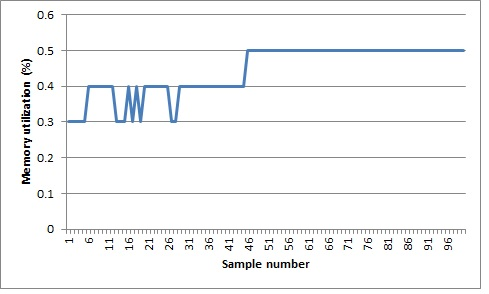
\includegraphics[width=100mm]{figures/scheme5_mem_util}
	\caption{Memory Utilization Footprint}
	\label{fig:mm:scheme5_mem_util}
\end{figure}


\subsection{Memory Transfer Bandwidth}
\label{ss:mm:scheme5:bw_util}
Memory footprint is reduced compared to the Scheme-3, leading to a smaller amount of operating data set per core. Private L1 cache and shared L2 cache can hold large portion of the operating data set, reducing memory transfer between SDRAM to core and so reducing memory transfer bandwidth. The lowest recorded memory transfer bandwidth by running the STREAM benchmark as a background task is listed in Table \ref{tbl:mm:scheme5_mem_bw}. Peak memory transfer bandwidth of the Radar application is measured as 30.3\% of the available 1048MiB/s.

\begin{table}[h!]
	\centering
	\begin{tabular}{|l|l|} 
	 \hline
	 \textbf{Function} & \textbf{Best Rate [MiB/s]} \\
	 \hline
	 Copy & 729.9 \\ \hline
	\end{tabular}
	\caption{Lowest Recorded Memory Transfer Bandwidth of the STREAM Benchmark}
	\label{tbl:mm:scheme5_mem_bw}
\end{table}

\begin{align*}
\label{aa:scheme4:mem_bw}
	BW_{p} &= BW_{i} - BW_{l} \\
	&= 1048 - 729.9 =  318.1 \: MiB/s \\
	&= \frac{318.1}{1048} = 30.3 \% \stepcounter{equation}\tag{\theequation} 
\end{align*}

\subsection{Summary}
\label{ss:mm:scheme5:summary}

Processing latency of 1.92x Dwell time and peak CPU utilization of 50.8\% are healthy values for Air to Air Mode Radar processor. It leaves remaining 49\% of the CPU utilization to accommodate future development. In fact, 8 CPUs are sufficient to give same processing latency. More CPUs are used to improve the utilization. Figure \ref{fig:mm:scheme5_summary} shows the relationship between number of CPUs used and their utilization without affecting the latency values. Any combination of the CPU sets can be chosen to achieve desired CPU utilization. Selecting 10 CPUs for burst processing and 1 CPU for correlation processing will have peak CPU utilization of 61\% and 1.92x dwell latency, leaving rest of the 13 CPUs for A/G mode processing in an IMA processor architecture. A comparison of  Scheme-1, Acceptable values and Scheme-4 is listed in Table \ref{tbl:mm:scheme5_comparison}.

\begin{figure}[h!]
	\centering
	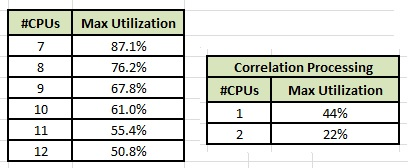
\includegraphics[width=90mm]{figures/scheme5_summary}
	\caption{Relationship Between Number of CPUs and Utilization}
	\label{fig:mm:scheme5_summary}
\end{figure}

\begin{table}[h!]
	\centering
	\begin{tabular}{|l|l|l|l|} 
	 \hline
	 \textbf{Parameter} & \textbf{Scheme-1} & \textbf{Acceptable Values} & \textbf{Scheme-4}\\
	 \hline
	 Dwell latency &  14.96 & 2 & 1.97 \\ \hline
	 CPU utilization & 75.5\% & \textless 50\% & 50.8\% \\ \hline
	 Memory Utilization & 7\% & \textless 50\%  & 0.5\% \\ \hline
	 Memory transfer bandwidth & NA & \textless 50\% & 30\%  \\ \hline
	\end{tabular}
	\caption{Comparison of Scheme-1 vs Acceptable Values vs Scheme-4}
	\label{tbl:mm:scheme5_comparison}
\end{table}

\section{Overview}
The Baseline Analysis has been observed to spot the latency contributors, bottlenecks and data dependencies. Upsides and downsides are evaluated to bring up the best scheduling scheme. Examined information have been supported in the design decisions of the scheduling scheme. Two new schemes are proposed to reduce the processing latency and they are validated via implementation. \vspace*{0.2cm}

Scheme-3 makes use of the fact that, the bursts in a Dwell can be processed independently until the Thresholding and Detection stage. This phenomenon skips waiting time in Beam-forming, Pulse compression, FFT, CFAR, Thresholding and Detection stage. This can be called as coarse grained parallelism. A dedicated processor is assigned for Correlation processing, without changing the execution method. Final outcome of the Scheme-3 is 4x Dwell time latency with 66\% CPU utilization. \vspace*{0.2cm}

Every burst data has large amount of fine grained parallelism. Four channel processing of a burst is done independently in Scheme-4, saving the waiting time for the other channel processing.  Correlation processing poses a bottleneck as the serial execution requires 1.5x Dwell time. Further, it is also parallelised and executed in dedicated CPUs. Deemed 2x Dwell time processing latency is achieved along with 50.8\% CPU utilization, provided 13 CPUs are performing computation. From the Table \ref{tbl:mm:scheme5_comparison} data, speed-up of the Scheme-4 compared to the best scheme(Scheme-1) in the Baseline Analysis is drawn as follows. \\

\begin{figure}[h!]
\centering
	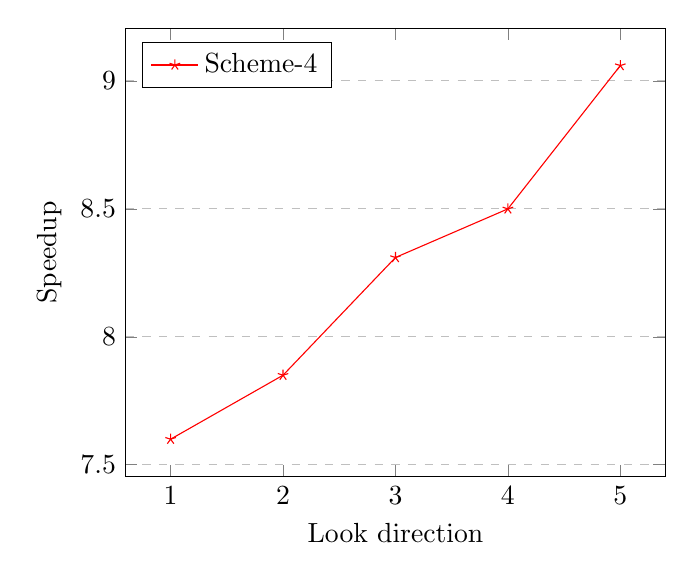
\begin{tikzpicture}
		\begin{axis}[
			xlabel={Look direction},
			ylabel={Speedup},
			legend pos=north west,
			ymajorgrids=true,
			grid style=dashed,
		]
		\addplot[color=red, mark=star,]
			coordinates {
				(1, 7.6) (2, 7.85) (3, 8.31) (4, 8.50) (5, 9.06)
			};
		\legend{Scheme-4}
	\end{axis}
\end{tikzpicture}
\caption{Speed-up, Scheme-4 vs Scheme-1}
\label{mm:scheme5_speedup}
\end{figure}

The best results of the Baseline Analysis are 75.5\% peak CPU utilization and 15x Dwell time latency, provided 12 CPUs are executing the Radar processing algorithm. For the same utilization value, Scheme-4 needs only 9 CPU resources and delivers acceptable latency of 2x Dwell time.

